\chapter{Organomagnesium Reagents}\label{ch:b1:organomagnesium}

Most useful organic molecules have more carbon atoms than any cheap
starting material, and the central problem of synthesis is to join two
carbon skeletons by a new C--C bond. In a carbon compound, carbon is
almost always the electron-poor partner of a bond --- to oxygen, to a
halogen --- and two electron-poor carbons do not react with each other.
At the turn of the twentieth century a reagent made in one flask from a
halogenoalkane and magnesium turned this around: its carbon is electron
rich, a \omterm{def:b1:electronic-effects:nucleophile}{nucleophile} that attacks the carbon of a carbonyl group. With it,
alcohols of almost any skeleton can be built from smaller pieces. This
chapter shows how the reagent is prepared, why it needs a perfectly dry
flask, what it adds to, and how to plan with it.

\begin{recall}
\omterm{def:b1:periodicity:electronegativity}{Electronegativity} (\cref{ch:b1:periodicity}); \omterm{def:b1:lewis-resonance-vsepr:lewis-acid}{Lewis acids} and bases and
the \omterm{def:b1:lewis-resonance-vsepr:lewis-acid}{dative bond} (\cref{ch:b1:lewis-resonance-vsepr}); \omterm{def:b1:electronic-effects:nucleophile}{nucleophiles},
\omterm{def:b1:electronic-effects:nucleophile}{electrophiles}, \omterm{def:b1:electronic-effects:curly-arrow}{curly arrows} and the $\mathrm{p}K_a$ scale of organic
species (\cref{ch:b1:electronic-effects}); the class of an alcohol
(primary, secondary, tertiary) follows that of its carbon.
\end{recall}

\section{Preparing a Grignard reagent}

\begin{definition}[Organometallic compound, Grignard reagent]\label{def:b1:organomagnesium:organometallic}
An \emph{organometallic compound}\index{organometallic compound} contains
at least one carbon--metal bond. An \emph{organomagnesium
compound}\index{organomagnesium compound} has a C--Mg bond; the
\emph{Grignard reagent}\index{Grignard reagent} \ce{RMgX} (X = Cl, Br, I),
prepared from a halogenoalkane or halogenoarene and magnesium in an ether,
\ce{R-X + Mg -> R-MgX}, is the most common.
\end{definition}

The magnesium inserts itself into the C--X bond. The ether is not an
innocent solvent: magnesium in \ce{RMgX} has only four \omterm{def:b1:quantum-numbers:configuration}{valence electrons}
around it, and two ether molecules give it their \omterm{def:b1:lewis-resonance-vsepr:lewis}{lone pairs}, completing
its octet and keeping the reagent in solution.

\begin{omfigure}
\begin{tikzpicture}[font=\small]
  \node (mg) at (0,0) {Mg};
  \node (r) at (-1.5,0) {R};
  \node (x) at (1.5,0) {Br};
  \node (o1) at (0,1.45) {O};
  \node (o2) at (0,-1.45) {O};
  \draw[thick] (r) -- (mg) -- (x);
  \draw[thick, ->, omDef] (o1) -- (mg);
  \draw[thick, ->, omDef] (o2) -- (mg);
  \draw (o1) -- ++(-0.8,0.45) node[left] {\ce{CH3CH2}};
  \draw (o1) -- ++(0.8,0.45) node[right] {\ce{CH2CH3}};
  \draw (o2) -- ++(-0.8,-0.45) node[left] {\ce{CH3CH2}};
  \draw (o2) -- ++(0.8,-0.45) node[right] {\ce{CH2CH3}};
  \node[align=left, anchor=west] at (3.2,0) {two ether molecules give\\a lone pair each (blue):\\tetrahedral magnesium,\\an octet of electrons};
\end{tikzpicture}

{\small A \omterm{def:b1:organomagnesium:organometallic}{Grignard reagent} in ethoxyethane (diethyl ether). The
oxygen--magnesium \omterm{def:b1:lewis-resonance-vsepr:lewis-acid}{dative bonds} explain why the reagent forms only in an
ether or a similar \omterm{def:b1:lewis-resonance-vsepr:lewis-acid}{Lewis base}.}
\end{omfigure}

\begin{method}[Preparing a Grignard reagent]\label{met:b1:organomagnesium:prepare}
\begin{enumerate}
  \item Dry all glassware in an oven; fit the condenser with a drying
        tube of calcium chloride; use an anhydrous ether.
  \item Put the magnesium turnings and a little ether in a three-necked
        flask fitted with condenser, addition funnel and stirrer.
  \item Add a small portion of the halide; when the reaction starts
        (cloudiness, gentle boiling of the ether), add the rest dropwise
        at a rate that keeps a gentle reflux.
  \item Use the solution at once, in the same dry apparatus.
\end{enumerate}
\end{method}

\begin{omfigure}
\begin{tikzpicture}[font=\small]
  \pic at (0,-0.05) {stirrer};
  \pic (f) at (0,0.05) {threeneck={0.35}{omDef!14}};
  \pic at (f-c) {condenser};
  \pic at ($(f-c)+(0,3.2)$) {guardtube};
  \pic[rotate=25] at (f-l) {dropfunnel={0.5}{orange!20}};
  \fill[black!45, rotate around={-25:(f-r)}] ($(f-r)+(-0.17,0)$) rectangle ++(0.34,0.3);
  \draw[->] (2.4,0.9) node[right] {Mg turnings in dry ether} -- (0.6,0.6);
  \draw[->] (-3.0,3.9) node[left, align=right] {halide in ether,\\added dropwise} -- (-1.8,3.4);
  \draw[->] (1.8,5.3) node[right] {condenser (water)} -- (0.45,4.8);
  \draw[->] (1.8,6.6) node[right] {calcium chloride drying tube} -- (0.3,6.4);
  \draw[->] (2.4,-0.2) node[right] {magnetic stirrer} -- (1.3,-0.2);
\end{tikzpicture}

{\small Apparatus for a Grignard reaction: everything that air can reach
is dried. The water vapour of the air is stopped by the drying tube; the
condenser returns the boiling ether to the flask.}
\end{omfigure}

\begin{inthelab}[A reaction that must start]
A Grignard preparation sometimes refuses to start: the magnesium is
covered with a film of oxide. Crushing a turning with a glass rod, adding
a \omterm{def:b1:crystals-metals:crystal}{crystal} of iodine, or warming the flask locally exposes fresh metal.
Once started, the reaction is exothermic and the ether boils on its own;
the addition is then slowed so that it does not boil over. Ethoxyethane
boils at \qty{35}{\celsius} and its vapour is highly flammable: no flame
anywhere in the laboratory, and an ice bath at hand.
% ledger: bp:diethylether
\end{inthelab}

\section{A strong base and a nucleophile}

\begin{definition}[Polarity inversion]\label{def:b1:organomagnesium:umpolung}
The \omterm{def:b1:periodicity:electronegativity}{electronegativity} of magnesium (1.31) is much lower than that of
carbon (2.55): in \ce{R-MgX} the C--Mg bond is polarised with the negative
end on carbon, which behaves as a \omterm{def:b1:electronic-effects:intermediates}{carbanion}. In the halide \ce{R-X} the
same carbon was positive (X: 2.96 for Br). Turning an electrophilic carbon
into a nucleophilic one is a \emph{polarity inversion}\index{polarity inversion}.
% ledger: en:Mg, en:C, en:Br
\end{definition}

\begin{proposition}[Grignard reagents are destroyed by acidic hydrogens]\label{prop:b1:organomagnesium:base}
A \omterm{def:b1:organomagnesium:organometallic}{Grignard reagent} reacts \omterm{def:b1:extent-q-and-k:quantitative}{quantitatively} with water, alcohols, carboxylic
acids, amines with N--H bonds and terminal alkynes, giving the alkane
\ce{R-H}: \ce{RMgX + H2O -> R-H + Mg(OH)X}.
\end{proposition}

\begin{proof}
The carbanion-like carbon is the base of the couple \ce{R-H}/\ce{R^-}, and
alkanes are by far the weakest acids of organic chemistry: no proton can
be measured to leave them in water, where hydroxide is the strongest base
that can exist (\cref{ch:b1:predominant-reaction}, levelling). Any acid
of the list is much stronger, and the proton transfer to \ce{R^-} has an
enormous constant: it is complete and fast.
\end{proof}

This is the reason for the dry apparatus: a drop of water destroys an
equal amount of reagent. Turned into an advantage, \ce{CH3CH2MgBr + D2O}
puts a deuterium atom exactly where the bromine was.

\section{Additions to carbonyl compounds and carbon dioxide}

The carbon of a C=O group is electrophilic
(\cref{ch:b1:electronic-effects}). The \omterm{def:b1:organomagnesium:organometallic}{Grignard reagent} adds its R group
to it, the C=O $\pi$ pair going to oxygen; an acidic work-up then
protonates the alkoxide.

\begin{omfigure}
\setchemfig{atom sep=2.1em}
\schemestart
\chemfig{@{r}R-[@{rm}]MgBr}
\+
\chemfig{@{cc}C(-[:150]R')(-[:210]R'')=[@{co}]@{o}O}
\arrow{->}
\chemfig{C(-[:150]R')(-[:210]R'')(-[2]R)-O^{-}}
\chemfig{\phantom{.}}\chemfig{^{+}MgBr}
\arrow{->[\ce{H3O+}]}
\chemfig{C(-[:150]R')(-[:210]R'')(-[2]R)-OH}
\schemestop
\chemmove{\draw[->, thick, shorten <=2pt, shorten >=2pt](rm) .. controls +(70:9mm) and +(180:7mm) .. (cc);
          \draw[->, thick, shorten <=2pt, shorten >=2pt](co) .. controls +(90:6mm) and +(90:6mm) .. (o);}
\par\vspace{6pt}

{\small Addition of a \omterm{def:b1:organomagnesium:organometallic}{Grignard reagent} to a ketone (or an aldehyde,
$\mathrm{R''} = \mathrm{H}$): the C--Mg pair forms the new C--C bond while the C=O $\pi$
pair goes to oxygen; the magnesium alkoxide is protonated by dilute acid
in a separate step.}
\end{omfigure}

\begin{proposition}[Alcohols from carbonyl compounds]\label{prop:b1:organomagnesium:carbonyl-addition}
After acidic work-up, a \omterm{def:b1:organomagnesium:organometallic}{Grignard reagent} \ce{RMgX} gives: with methanal, a
primary alcohol \ce{RCH2OH}; with another aldehyde $\mathrm{R'CHO}$, a secondary
alcohol $\mathrm{RR'CHOH}$; with a ketone $\mathrm{R'COR''}$, a tertiary alcohol
$\mathrm{RR'R''COH}$. The new C--C bond joins R to the former carbonyl carbon.
\end{proposition}

\begin{proof}
The carbonyl carbon keeps its two substituents and gains R and an OH
(from the alkoxide oxygen): methanal brings two H, an aldehyde one H and
one carbon group, a ketone two carbon groups. The class of the alcohol is
the number of carbon groups on that carbon: one, two or three.
\end{proof}

\begin{proposition}[Carboxylic acids from carbon dioxide]\label{prop:b1:organomagnesium:co2}
A \omterm{def:b1:organomagnesium:organometallic}{Grignard reagent} poured onto solid carbon dioxide gives, after
acidification, the carboxylic acid \ce{RCOOH} with one more carbon:
\ce{RMgX + CO2 -> RCOOMgX}, then \ce{RCOOMgX + H3O+ -> RCOOH + Mg^2+ + X- + H2O}.
\end{proposition}

\begin{proof}
\ce{CO2} is a carbonyl compound whose carbon is attacked like that of a
ketone; the carboxylate formed is too unreactive to add a second R group
in these conditions (a negatively charged carbonyl is a poor
\omterm{def:b1:electronic-effects:nucleophile}{electrophile}). Acid protonates it.
\end{proof}

\section{Building carbon skeletons}

\begin{method}[Planning an alcohol]\label{met:b1:organomagnesium:plan-alcohol}
\begin{enumerate}
  \item Find the carbon bearing the OH in the target alcohol.
  \item Choose one of its carbon groups as R (it will come from the
        \omterm{def:b1:organomagnesium:organometallic}{Grignard reagent}, prepared from \ce{R-Br}); the rest of the
        molecule, with that carbon as a C=O, is the carbonyl partner.
  \item List the possible choices (one per carbon group) and prefer the
        one with simple, available reagents.
  \item Check that neither partner carries an acidic hydrogen or a second
        carbonyl that would react too.
\end{enumerate}
\end{method}

\begin{example}[2-Phenylbutan-2-ol]\label{ex:b1:organomagnesium:plan}
The carbon bearing OH carries a phenyl, a methyl and an ethyl group.
Three choices: phenylmagnesium bromide with butan-2-one; methylmagnesium
bromide with 1-phenylpropan-1-one; ethylmagnesium bromide with
1-phenylethan-1-one (acetophenone). All three work; the last uses two of
the commonest reagents.
\end{example}

\begin{history}[Victor Grignard]
\begin{minipage}[t]{0.2\linewidth}\vspace{0pt}
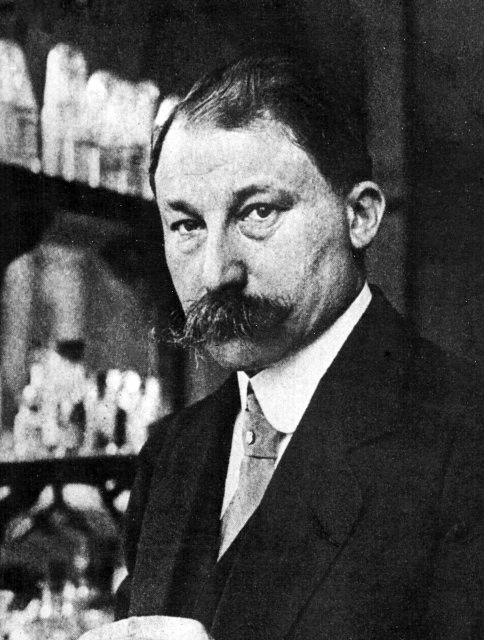
\includegraphics[width=\linewidth]{images/book2/grignard.jpg}
\end{minipage}\hfill
\begin{minipage}[t]{0.76\linewidth}\vspace{0pt}
The reagent bears the name of Victor Grignard, who, as a doctoral student
at the turn of the twentieth century, found that magnesium dissolves in
an ether solution of a halogenoalkane and that the solution adds to
carbonyl compounds. Its simplicity --- one metal, one solvent, one flask
--- made it the most used carbon--carbon bond-forming reaction of the
century, and earned its discoverer a Nobel Prize in Chemistry.
(Photograph, public domain, Wikimedia Commons.)
\end{minipage}
\end{history}

\section{Exercises}

\begin{exercise}[$\star$]\label{exo:b1:organomagnesium:1}
Write the preparation of ethylmagnesium bromide and of
phenylmagnesium bromide. Give the polarisation of the C--Br bond and of
the C--Mg bond, with the electronegativities.
\end{exercise}

\begin{exercise}[$\star$]\label{exo:b1:organomagnesium:2}
What does methylmagnesium iodide give with: water; ethanol; ethanoic
acid; deuterium oxide \ce{D2O}? Write the equations.
\end{exercise}

\begin{exercise}[$\star$]\label{exo:b1:organomagnesium:3}
Give the product (after acidic work-up) of ethylmagnesium bromide with
methanal, ethanal, propanone, benzaldehyde and carbon dioxide. Give the
class of each alcohol.
\end{exercise}

\begin{exercise}[$\star$]\label{exo:b1:organomagnesium:4}
Why must 4-bromobutan-1-ol not be used to prepare a \omterm{def:b1:organomagnesium:organometallic}{Grignard reagent}?
\end{exercise}

\begin{exercise}[$\star\star$]\label{exo:b1:organomagnesium:5}
Write the mechanism of the addition of methylmagnesium bromide to ethanal
and of the work-up, with \omterm{def:b1:electronic-effects:curly-arrow}{curly arrows}. Is the product \omterm{def:b1:stereochemistry-in-depth:stereocentre}{chiral}? Is it
obtained as a single enantiomer? Why?
\end{exercise}

\begin{exercise}[$\star\star$]\label{exo:b1:organomagnesium:6}
Propose two ways to prepare 3-methylpentan-3-ol from a \omterm{def:b1:organomagnesium:organometallic}{Grignard reagent}
and a ketone.
\end{exercise}

\begin{exercise}[$\star\star$]\label{exo:b1:organomagnesium:7}
How would you prepare 2-methylpropanoic acid from 2-bromopropane? Compute
the mass of acid obtained from \qty{12.3}{g} of bromide at
\qty{70}{\percent} \omterm{def:b1:extent-q-and-k:fractional-extent}{yield} ($M$: \ce{C3H7Br} \qty{123.0}{g/mol}, \ce{C4H8O2}
\qty{88.0}{g/mol}).
\end{exercise}

\begin{exercise}[$\star\star$]\label{exo:b1:organomagnesium:8}
A careless student prepares phenylmagnesium bromide from
\qty{0.0500}{mol} of bromobenzene in ether containing \qty{0.18}{g} of
water. What fraction of the reagent is destroyed? Which product forms?
\end{exercise}

\begin{exercise}[$\star\star$]\label{exo:b1:organomagnesium:9}
Biphenyl, \ce{C6H5-C6H5}, is a by-product of the preparation of
phenylmagnesium bromide. Propose how it forms, and why slow addition of
bromobenzene to excess magnesium limits it.
\end{exercise}

\begin{exercise}[$\star\star\star$]\label{exo:b1:organomagnesium:10}
Plan two syntheses of 1-phenylethan-1-ol from a \omterm{def:b1:organomagnesium:organometallic}{Grignard reagent}, and a
synthesis of 2-phenylpropan-2-ol. For each, name the halide that gives the
reagent.
\end{exercise}

\begin{exercise}[$\star\star\star$]\label{exo:b1:organomagnesium:11}
Explain why the \omterm{def:b1:organomagnesium:organometallic}{Grignard reagent} and the carbonyl compound must be mixed
in the order chosen in the problem below, and why the work-up is done
with cold dilute acid rather than with water alone.
\end{exercise}

\begin{exercise}[$\star\star\star$]\label{exo:b1:organomagnesium:12}
A \omterm{def:b1:organomagnesium:organometallic}{Grignard reagent} made from \qty{0.100}{mol} of a bromide is titrated:
an aliquot is poured into excess water, and the basic magnesium salt
formed is titrated by hydrochloric acid: scaled to the whole solution,
\qty{0.088}{mol} of acid are needed. Explain the principle and give the \omterm{def:b1:extent-q-and-k:fractional-extent}{yield} of the
preparation.
\end{exercise}

\section{Problem: Triphenylmethanol}

\begin{problem}[{Weekend problem --- preparing phenylmagnesium bromide,
its addition to benzophenone, the work-up, and the yield of
triphenylmethanol}]
\label{pb:b1:organomagnesium:1}
In a dry three-necked flask, \qty{0.535}{g} of magnesium and
\qty{3.14}{g} of bromobenzene in anhydrous ethoxyethane give
phenylmagnesium bromide. A solution of \qty{3.28}{g} of benzophenone,
\ce{(C6H5)2CO}, in the same ether is then added dropwise. After work-up
with cold dilute sulfuric acid, extraction and recrystallisation,
\qty{3.75}{g} of pure triphenylmethanol, \ce{(C6H5)3COH}, are obtained,
and \qty{0.15}{g} of biphenyl are separated. Molar masses (\unit{g/mol}):
Mg 24.3, \ce{C6H5Br} 156.9, \ce{C13H10O} 182.0, \ce{C19H16O} 260.0,
\ce{C12H10} 154.0, \ce{C7H6O2} 122.0.

\medskip
\noindent\textbf{Part I --- Phenylmagnesium bromide.}
\begin{enumerate}
  \item Write the equation of the preparation.
  \item Compute the amounts of magnesium and bromobenzene. Which is in
        excess?
  \item Why must the apparatus be dry? Write the reaction with water.
  \item What is the role of the drying tube?
  \item Why is the ether essential, beyond dissolving the reagents?
  \item Biphenyl comes from the reaction of the reagent with bromobenzene.
        Write it and compute the amount of bromobenzene lost to it.
\end{enumerate}

\medskip
\noindent\textbf{Part II --- The addition.}
\begin{enumerate}[resume]
  \item Compute the amount of benzophenone.
  \item Write the mechanism of the addition with \omterm{def:b1:electronic-effects:curly-arrow}{curly arrows}.
  \item Which reagent limits the formation of triphenylmethanol? Take
        Part I into account.
  \item Is triphenylmethanol \omterm{def:b1:stereochemistry-in-depth:stereocentre}{chiral}? Justify.
  \item Why is the benzophenone added to the reagent, and not the reverse?
  \item What would a trace of water in the benzophenone solution do?
\end{enumerate}

\medskip
\noindent\textbf{Part III --- Work-up.}
\begin{enumerate}[resume]
  \item Write the protonation of the alkoxide.
  \item Why use cold dilute acid rather than water alone?
  \item Where are triphenylmethanol and the magnesium salts after
        extraction with ether?
  \item How is biphenyl separated from triphenylmethanol? (Biphenyl is far
        more soluble in cold light petroleum.)
  \item Which test confirms the purity of the \omterm{def:b1:crystals-metals:crystal}{crystals}?
  \item Triphenylmethanol survives cold dilute acid, but dissolves in
        concentrated sulfuric acid to give a deep yellow \omterm{def:b1:electronic-effects:intermediates}{carbocation}.
        Write its formation and explain its stability (compare with
        \cref{ch:b1:electronic-effects}).
\end{enumerate}

\medskip
\noindent\textbf{Part IV --- \omterm{def:b1:extent-q-and-k:fractional-extent}{Yield}, and another product.}
\begin{enumerate}[resume]
  \item Compute the amount of triphenylmethanol obtained.
  \item Compute the \omterm{def:b1:extent-q-and-k:fractional-extent}{yield} relative to the limiting reagent.
  \item Suggest two causes of loss.
  \item If the reagent of Part I (corrected for biphenyl) had been poured
        onto solid carbon dioxide instead, which product would form?
  \item Compute the theoretical mass of that product.
  \item Write the equation of that carboxylation.
  \item State the \omterm{def:b1:extent-q-and-k:fractional-extent}{yield} of triphenylmethanol, in per cent.
\end{enumerate}
\end{problem}
